\documentclass[12pt,a4paper]{article}
\usepackage{fullpage}
\pagestyle{plain}
\usepackage{amsmath}
\usepackage{graphicx}
\usepackage{indentfirst}
\graphicspath{{./img}}
% choose any of the following packages to support AmsTeX
%\usepackage{amsmath,amssymb,amsfonts,mathrsfs,mathptm,bm,mathtools}
% choose the following package to insert eps figures
% for png, jpg or pdf figures, use pdflatex
%\usepackage{graphicx}

\newcommand{\question}[1]{\bigskip\noindent{\textbf{Q{#1} solution}}}

% set HW number
\newcommand{\HWnum}{2}
% specify first and last name and the ID number of students in the group
% append asterix to indicate who is making the submission
\newcommand{\StudentA}{Hanggang Zhu$^\ast$, 3200110457}
\newcommand{\StudentB}{Suhao Wang, 3200110777}
\newcommand{\StudentC}{Lumeng Xu 3200110184}

% ===============================================================
\begin{document}

%%% header
{\noindent \rule{\linewidth}{0.2mm}}\\
\noindent{ECE 374, ZJUI, Spring 2023\hfill%
  \textbf{\large H{}W\HWnum\ Solutions} \hfill \today\smallskip}

\noindent{\hfill \StudentA, \StudentB, and \StudentC \hfill}
\\[-0.2cm]{\noindent \rule{\linewidth}{0.2mm}}
%%% end header



\question{4.A}
\\As $(0+1)^\ast$ represents any strings, it means any string can be 
in front of $1011$. And $1011$ appears in the end ensures that all strings end in $1011$.
\\\textbf{Answer:} $(0+1)^\ast 1011$

\question{4.B}
\\We should represent all strings except 11, so we just list out all 
other strings of length less or equal to 2, and all strings of length greater than 2.\\
\textbf{Answer:} $\epsilon+0+1+00+01+10+(0+1)^3(0+1)^\ast$

\question{4.C}
\\As the strings contain 101 or 010 as a substring, we should add 
any strings before and after (010+010) to make sure we represent all 
the strings.
\\\textbf{Answer:} $(0+1)^\ast (101+010)(0+1)^\ast$

\question{4.D}
\\As the strings should contain 111 and 000 as a subsequence, it should contain both 111 and 000 as a subsequence at the same time. So, we can list all the possible combinations containing 111 and 000 as a subsequence. The number of combinations is ${6 \choose 3} = 20$.The regular expression can be represented by inserting $(0+1)^*$ in between any two characters.
\\\textbf{Answer:} Let A be the set containing all combinations with 3 $1$s and 3 $0$s.
$A=\{000111, 001011,010011 ...\}$ with 20 elements in total. The regular expression is formed by inserting $(0+1)^*$ between any two characters as well as end and start of the string.

\question{4.E}
\\As we should represent all strings that don't contain 111 as a 
substring, we should avoid the appearance of 111. So, we can add 0
after $(\epsilon+1+11)$, and it can appear any times before $(\epsilon+1+11)0^\ast$.
\\\textbf{Answer:} $((\epsilon+1+11)0)^\ast(\epsilon+1+11)0^\ast$

\question{4.F}

Strings not containing subsequence $000$ is equivalent to having at most two $0$s. The regular expression simply consider three cases.\\
\textbf{Answer:} $1^* + 1^*01^* + 1^*01^*01^*$

\question{4.G}

The string can also be interpreted as string whose substring with no $11$s come before substring with no $00$s.String with no $11$:$(\epsilon + 1)(0(\epsilon + 1 ))^*$. String with no $00$: $(\epsilon + 0)(1(\epsilon + 0))^*$.Concatenate them and simply.\\
\textbf{Answer:} $(\epsilon + 1)(0(\epsilon + 1))^*(1(\epsilon + 0))^*$


\question{4.H}

Strings not containing subsequence $010$ means that $1$ can't be in the middle of two $0$s. So $1$ must be on one side of $0$s.\\
\textbf{Answer:} $1^*0^*1^*$

\question{4.I}

Given four continuous $0$s, we can't put $1$s between every cut of these $0$s. If we remove these $1$s, we can get $0^*1^*0^*1^*0^*$(remove one $1$s) or $0^*1^*0^*$(remove two $1$s) and $0^*$(remove three $1$s). They are all included in the case of $0^*1^*0^*1^*0^*$. We generalize it by adding $1$s at two sides.\\
\textbf{Answer:}$1^*0^*1^*0^*1^*0^*1^*$

\question{4.J}

Strings not containing subsequence $10$ means $0$s must come before $1$s.\\
\textbf{Answer:}$0^*1^*$


\question{5.A}

The DFA is drawn in figure \ref{fig:DFA}. The DFA accepts all strings that contain an even number of 0s and an even number of 1s. Each state represents whether the numbers of 0s and 1s are even or odd. The front letter represents whether the number of 0 is even or not, and the latter number represents whether the number of 1 is even or not.

As we design in the DFA, these states represent all possible patterns of strings in terms of odd or even number of $1$s and $0$s. But only state $q_0(E,E)$ is accpeted,which means it only accept every string with even number of $0$s and $1$s and nothing else.

\begin{figure}[hbt!]
  \centering
  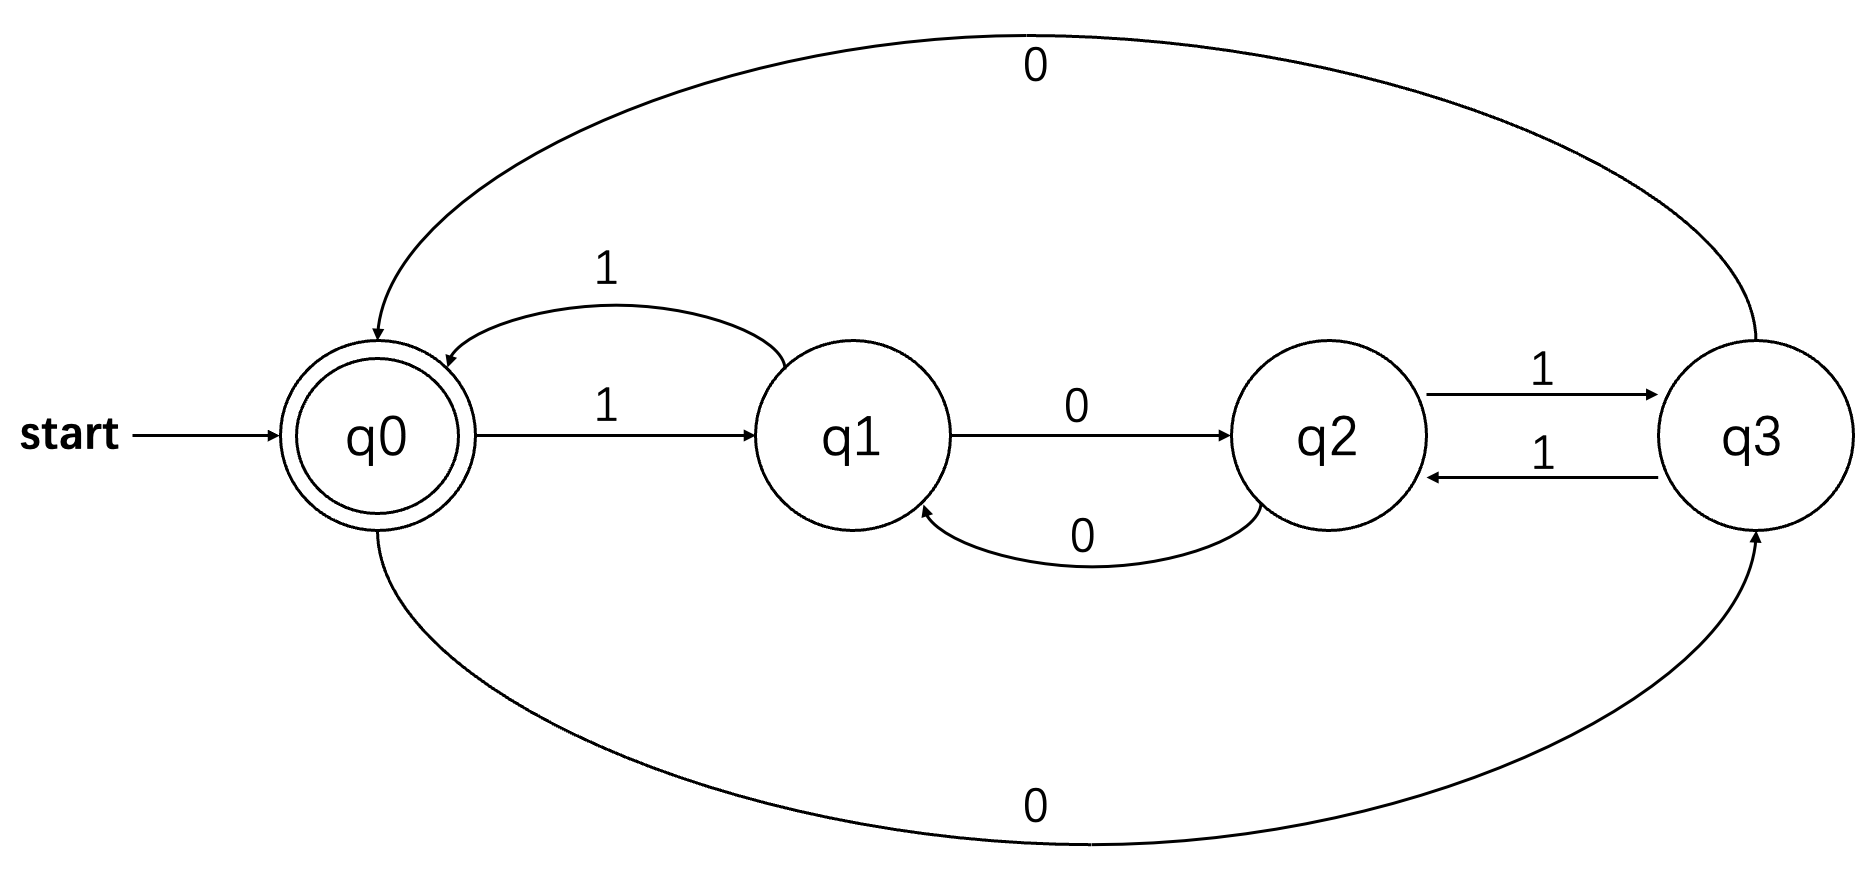
\includegraphics[width = 0.7\textwidth]{img/374hw2.png}
  \caption{Q5.A DFA}
  \label{fig:DFA}
\end{figure}


\question{5.B}

To find regular expression with even number of $0$s and even number of $1$s, first consider the simple case where the strings do not contain any consecutive $1$s and $0$s. In this case, the regular expression is $(1010)^* + (0101)^*$. The examples are $01010101...$ and $10101010...$. We can extentily easily by allowing patterns like $01101001$. So we extend the regular expression to $((01+10)(01+10))^*$. For now we allow at most 2 consecutive $0$s and $1$s. We can allow any number of consecutive $0$ and $1$s by cut regular expressions using (00+11)*. Then regular expression becomes $((00+11)^*(01+10)(00+11)^*(01+10)(00+11)^*)^*$, which is the answer.

The correctness of this regular expression lies in the assurance that number of $1$s and $0$s are even. It generalizes by considering cases where there's no consecutive characters, allowing 2 consecutive characters and no limit no consecutive characters.

\question{6.A}

\noindent For language $L = L_1 \cap L_2 \cap L_3$, formally describe the DFM as  $M = (Q,\sum,\delta,s,A)$, where

$\bullet$ $Q = Q_1 \times Q_2 \times Q_3 = \{(q_1,q_2,q_3)\ \vline\ q_1 \in Q_1, q_2 \in Q_2, q_3 \in Q_3\}$

$\bullet$ $\delta:Q \times \sum \rightarrow Q \mbox{ ,where } \delta((q_1,q_2,q_3),a) = (\delta_1(q_1,a),\delta_2(q_2,a),\delta_3(q_3,a)) \mbox{ and } a \in \sum$

$\bullet$ $s = (s_1,s_2,s_3)$

$\bullet$ $A = A_1 \times A_2 \times A_3 = \{(q_1,q_2,q_3)\ \vline\ q_1 \in A_1, q_2 \in A_2, q_3 \in A_3\}$

\question{6.B}

For $\delta^*(q,w)$, we have the formal definition:

\begin{equation*}
\delta^*(q,w) = 
  \begin{cases}
    q & \mbox{, if } w = \epsilon, \\
    \delta^*(\delta(q,a),x) & \mbox{, if } w = ax
  \end{cases}
\end{equation*}

Now we prove by induction. 

$\bullet$ \textbf{Base case:} Let $w$ be an artibrary string of length 0. we get $w = \epsilon$. Then
\begin{align*}
\delta^*((q_1,q_2,q_3),w) &= \delta^*((q_1,q_2,q_3),\epsilon) \\
    &= (q_1,q_2,q_3) \\ 
    &= (\delta_1^*(q_1,\epsilon), \delta_2^*(q_2,\epsilon), \delta_3^*(q_3,\epsilon)) \\
    &= (\delta_1^*(q_1,w), \delta_2^*(q_2,w), \delta_3^*(q_3,w))
\end{align*}

$\bullet$ \textbf{Induction hypothesis:} For any string $w$ of length $n > 0$, we have that
\begin{equation*}
  \delta^*((q_1,q_2,q_3),w) = (\delta_1^*(q_1,w), \delta_2^*(q_2,w), \delta_3^*(q_3,w))
\end{equation*}

$\bullet$ \textbf{Inductive step:} Let $w$ be an artibrary string with length $n > 0$. Assume inductive hypothesis holds for all strings x of length $< n$. Then we have $w = ax$ for some string x with length $< n$ and $a \in \sum$. We have:
\begin{align*}
  \delta^*((q_1,q_2,q_3),w) &= \delta^*(\delta((q_1,q_2,q_3), a), x) &\mbox{(definition of $\delta^*(q,w)$) }\\
      &= \delta^*((\delta_1(q_1,a), \delta_2(q_2,a), \delta_3(q_3,a)), x) &\mbox{(definition of $\delta$ in Q6.A)}\\
      &= (\delta_1^*(\delta_1(q_1,a), x),\delta_2^*(\delta_2(q_2,a), x),\delta_3^*(\delta_3(q_3,a), x)) &\mbox{(induction hypothesis)}\\
      &= (\delta_1^*(q_1,w), \delta_2^*(q_2,w), \delta_3^*(q_3,w)) &\mbox{(definition of $\delta^*(q,w)$) }
\end{align*}

So, the equation is proved.


\question{6.C}\\

	$\bullet$ \textbf{intuition:} "w is in exactly two of {L1,L2,L3}" means that $w \in L = (L_1 \cap L_2 \cap \overline{L_3}) \cup ( L_1 \cap \overline{L_2} \cap L_3) \cup (\overline{L_1} \cap L_2 \cap L_3)$. ($\overline{L}$ means complement of L). Define $L4=(L_1 \cap L_2 \cap \overline{L_3})$, $L5=( L_1 \cap \overline{L_2} \cap L_3)$, $L6 = (\overline{L_1} \cap L_2 \cap L_3)$.


	$\bullet$ \textbf{complement result:}According to the theorem and proof in the lecture 3," Languages accepted by DFAs are closed under complement", we will know that for $M = (Q,\sum,\delta,s,A)$ such that $L=L(M)$, we can find $M' = (Q,\sum,\delta,s,Q \backslash A)$ that $\overline{L}=L(M')$. 


	$\bullet$ \textbf{intersection result:}According to the theorem and proof in the lecture 3 as well as what we prove in question 6.B, we will know that for $M = (Q,\sum,\delta,s,A)$ such that $L=L(M)$, we can formally describe the DFM for L4 as  $M4 = (Q_{4},\sum,\delta_{4},s_{4},A_{4})$, where

	$\bullet$ $Q_4 = Q_1 \times Q_2 \times \overline{Q_3} =  Q_1 \times Q_2 \times Q_3 =\{(q_1,q_2,q_3)\ \vline\ q_1 \in Q_1, q_2 \in Q_2, q_3 \in Q_3\}$

	$\bullet$ $\delta_4: \delta((q_1,q_2,\overline{q_3}),a) = \delta((q_1,q_2,q_3),a) = (\delta_1(q_1,a),\delta_2(q_2,a),\delta_3(q_3,a)) \mbox{ and } a \in \sum$

	$\bullet$ $s_4 = (s_1,s_2,\overline{s_3}) = (s_1,s_2,s_3)$

	$\bullet$ $A_4 = A_1 \times A_2 \times \overline{A_3} = A_1 \times A_2 \times Q3 \backslash A_3 = \{(q_1,q_2,q_3)\ \vline\ q_1 \in A_1$ and $q_2 \in A_2$ and $q_3 \in Q_3 \backslash A_3\}$\\
	{Do the similar work for L5 and L6, we will get:}\\


	$\bullet$ $Q_5 = Q_4 = Q_6 $

	$\bullet$ $\delta_5 = \delta_4 = \delta_6$

	$\bullet$ $s_5 = s_4 = s_6$

	$\bullet$ $A_5 = A_1 \times \overline{A_2} \times A_3 = \{(q_1,q_2,q_3)\ \vline\ q_1 \in A_1, q_2 \in Q_2 \backslash A_2, q_3 \in A_3\}$

	$\bullet$ $A_6 = \overline{A_1} \times A_2 \times A_3 = \{(q_1,q_2,q_3)\ \vline\ q_1 \in Q_1 \backslash A_1, q_2 \in A_2, q_3 \in A_3\}$


	$\bullet$ \textbf{complement result:}{Then we calculate the union of $L_4,L_5,L_6$ and finally get the answer: $M = (Q,\sum,\delta,s,A)$}\\
	
	$\bullet$ $Q = \{(q_1,q_2,q_3,q_1',q_2',q_3',q_1'',q_2'',q_3'')\ \vline\ q_1,q_1',q_1'' \in Q_1, q_2,q_2',q_2'' \in Q_2, q_3,q_3',q_3'' \in Q_3\}$

	$\bullet$ $\delta = (\delta_1(q_1,a),\delta_2(q_2,a),\delta_3(q_3,a),\delta_1(q_1',a),\delta_2(q_2',a),\delta_3(q_3',a),\delta_1(q_1'',a),\delta_2(q_2'',a),\delta_3(q_3'',a)) \mbox{ and } a \in \sum$

	$\bullet$ $s = (s_1,s_2,s_3,s_1',s_2',s_3',s_1'',s_2'',s_3'')$

	$\bullet$ $A = A_1 \times A_2 \times Q_3 \backslash A_3 \times A_1 \times Q_2 \backslash A_2 \times A_3 \times Q_1 \backslash A_1 \times A_2 \times A_3= \{(q_1,q_2,q_3,q_1',q_2',q_3',q_1'',q_2'',q_3'')\ \vline\ (q_1 \in A_1, q_2 \in A_2, q_3 \in Q_3 \backslash A_3)\quad  or \quad (q_1' \in A_1, q_2' \in Q_2 \backslash A_2, q_3' \in A_3) \quad or \quad  (q_1'' \in Q_1 \backslash A_1, q_2'' \in A_2, q_3'' \in A_3)\}$
	

		

\question{6.D}\\
	$\bullet$ \textbf{intuition:}Separate these three conditions, and then use our conclusion in B to intersect.


	$\bullet$ \textbf{Answer:}
Set $L_1=\left\{ w \ \vline\ w \notin L(M) \right\}$ and $L_2=\left\{w \ \vline\ \overline{w} \in L(M)\right\}$ and $L_3=\left\{w \ \vline\ 1^{|w|} \in L(M)\right\}$.


	Then $L1(M)=\overline{L(M)}$, so we can get:
	
	$\bullet$ $Q_1 = Q$

	$\bullet$ $\delta_1(q,a) = \delta(q,a) $

	$\bullet$ $s_1 = s$

	$\bullet$ $A_1 = Q \backslash A$\\

	And for $L2(M)$, we have:
	
	$\bullet$ $Q_2 = Q$

	$\bullet$ $\delta_2(q,1) = \delta(q,0), \quad \delta_2(q,0) = \delta(q,1) $

	$\bullet$ $s_2 = s$

	$\bullet$ $A_2 = A$\\

	And for $L3(M)$, we have:
	
	$\bullet$ $Q_3 = Q$

	$\bullet$ $\delta_3(q,1) = \left\{ \delta(q,0),\delta(q,1) \right\}, \quad \delta_3(q,0) = \emptyset $

	$\bullet$ $s_3 = s$

	$\bullet$ $A_3 = A$\\
	
	Finally, we can get $L' = L_1 \cap L_2 \cap L_3$ and use Q6.A to describe L' and so that we can describe the DFA and $n= \vline\ Q_1 \times Q_2 \times Q_3 \   \vline\ = \vline\ Q \times Q \times Q \ \vline\ $
	
	$\bullet$ $Q = Q_1 \times Q_2 \times Q_3 = \{(q_1,q_2,q_3)\ \vline\ q_1 \in Q_1, q_2 \in Q_2, q_3 \in Q_3\}$

	$\bullet$ $\delta:Q \times \sum \rightarrow Q \mbox{ ,where } \delta((q_1,q_2,q_3),a) = (\delta_1(q_1,a),\delta_2(q_2,a),\delta_3(q_3,a)) \mbox{ and } a \in \sum$

	$\bullet$ $s = (s_1,s_2,s_3)$

	$\bullet$ $A = A_1 \times A_2 \times A_3 = \{(q_1,q_2,q_3)\ \vline\ q_1 \in A_1, q_2 \in A_2, q_3 \in A_3\}$



\end{document}

